%________________________________________________________
\section{Batch analysis}
\label{Note:BATCH}

In this section, we will describe the batch framework. We will first describe the flow of the procedure; we dedicate a sub-section to describe in detail the integration of the \tag in the batch sessions. We will then use the next paragraphs to describe in detail the files needed to submit a batch job as well as the jdl syntax. Finally we will provide a snapshot of a jdl and we will mention how we can submit a job on the grid and how we can see at any time its status.

%________________________________________________________
\subsection{Overview of the framework}

\begin{figure}[ht!]
\begin{center}
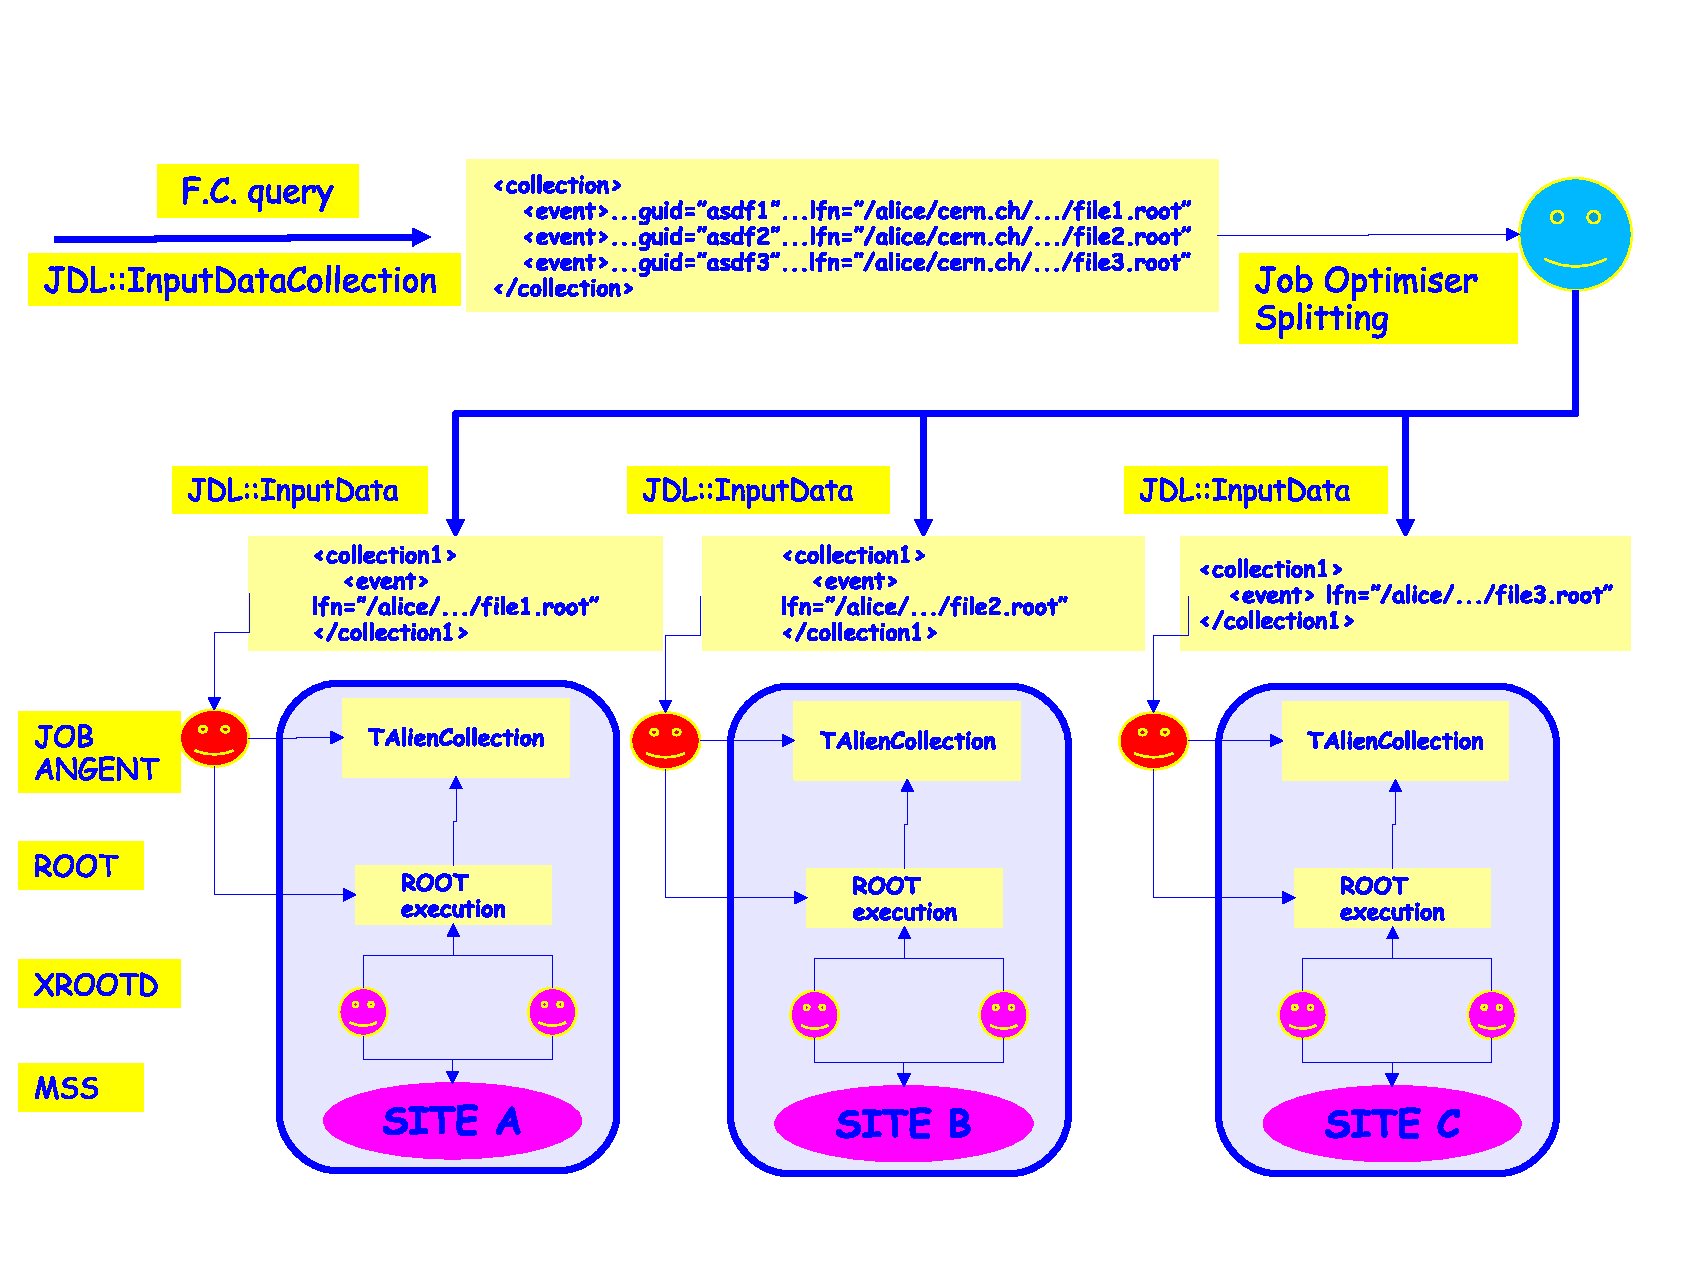
\includegraphics[height=0.5\textheight,width=0.7\textheight]{figures/Batch1.eps}
\end{center}
\caption{A schematic view of the flow of analysis in a batch session. Following the arrows, we have the initial xml collection which is listed in the jdl as an {\ttfamily InputDataCollection} field. The optimizer takes this xml and splits the master job into several sub-jobs while in parallel writing new xml collections on every worker node. Then the respective job agents on every site start a ROOT or IlcRoot session, read these new xml collections and interact with the xroot servers in order to retrieve the needed files. Finally, after the analysis is completed, a single output file is created for every sub-job.}
\label{Note:FigAnalsysisFlowBatch}
\end{figure}

Fig.\,\ref{Note:FigAnalsysisFlowBatch} shows the flow of a batch session \cite{Note:RefIlcenTutorial}. We start, as we have explained in section \ref{Note:FLOW}, by querying the file catalog and extracting a collection of files. This collection will be referenced by our jdl as an {\ttfamily InputDataCollection} field. Once we have created our jdl (a detailed description of the jdl syntax comes in the next sections) and all the files listed in it are in the proper place, we submit the job. The optimizer of the AliEn task queue parses the xml file and splits the master job into several smaller ones each one assigned to a different site. In parallel, a new xml collection is written on every site, containing the information about the files to be analyzed on every worker node.

The corresponding job agent of every site starts the execution of the ROOT (in case we use the combination ROOT + {\ttfamily par file}) or IlcRoot session, parses this new xml collection and interacts with the xroot servers in order to retrieve from the storage system the files that are listed inside these collections. The analysis of these different sets of files results into the creation of several output files, each one containing the output of a sub-job. The user is responsible to launch a post process, that will loop over the different output files in order to merge them (an example on how to merge output histograms will be described in the next section).


%________________________________________________________
\subsection{Using the \tag}

To use the \tag, we have to use some {\ttfamily \textbf{IlcRoot}} classes that are in the {\ttfamily \textbf{STEER}} module. The main classes, as described in a previous section (section \ref{Note:LOCAL}), are the {\ttfamily \textbf{IlcTagAnalysis}}, {\ttfamily \textbf{IlcRunTagCuts}} and {\ttfamily \textbf{IlcEventTagCuts}}. In order to use the \tag in a batch session, we need to perform an initial step described in Fig.\,\ref{Note:FigAnalysisFlow}: starting from a tag xml collection obtained by querying the file catalog, we define our selection criteria according to our physics analysis and we create a new xml collection having this time the information about the IlcESDs\footnote{The user should realize that the initial xml collection, named in the examples as {\ttfamily tag.xml}, held the information about the location of the tag files inside the file catalog. Instead what we create at this step is a new xml collection that will refer to the location of the ESD files.}. In this xml collection, we also list the events that satisfy the imposed selection criteria for every ESD file. The following lines show how we can generate a new xml collection (you can find these lines in the {\ttfamily \textbf{CreateXML.C}} macro inside the {\ttfamily \textbf{STEER}} module):

\vspace{0.5 cm}
\textbf{Usage of IlcRunTagCuts and IlcEventTagCuts classes}
\begin{lstlisting}[language=C++]
  // Case where the tag files are stored in the file catalog
  // tag.xml is the xml collection of tag files that was produced 
  // by querying the file catalog.
  TGrid::Connect("alien://"); 
  TAlienCollection* coll = TAlienCollection::Open("tag.xml");
  TGridResult* tagResult = coll->GetGridResult("");
  
  // Create a new IlcTagAnalysis object
  IlcTagAnalysis *tagAna = new IlcTagAnalysis(); 

  // Create a tag chain by providing the TGridResult
  // from the previous step as an argument
  tagAna->ChainGridTags(tagResult);

  //Usage of IlcRunTagCuts & IlcEventTagCuts classes//
  // Create a RunTagCut object
  IlcRunTagCuts *runCutsObj = new IlcRunTagCuts();
  runCutsObj->SetRunId(340);

  // Create an EventTagCut object
  IlcEventTagCuts *evCutsObj = new IlcEventTagCuts();
  evCutsObj->SetMultiplicityRange(2, 100);

  // Create the esd xml collection:the first argument is the 
  // collection name while the other two are the imposed criteria
  tagAna->CreateXMLCollection("global", runCutsObj, evCutsObj);
\end{lstlisting}


\vspace{0.5 cm}
\textbf{Usage of string statements}
\begin{lstlisting}[language=C++]
  // Case where the tag files are stored in the file catalog
  // tag.xml is the xml collection of tag files that was produced 
  // by querying the file catalog.
  TGrid::Connect("alien://"); 
  TAlienCollection* coll = TAlienCollection::Open("tag.xml");
  TGridResult* tagResult = coll->GetGridResult("");
  
  // Create a new IlcTagAnalysis object
  IlcTagAnalysis *tagAna = new IlcTagAnalysis(); 

  // Create a tag chain by providing the TGridResult
  // from the previous step as an argument
  tagAna->ChainGridTags(tagResult);

  //Usage of string statements//
  const char* runCutsStr = "fIlcRunId == 340";
  const char* evCutsStr = "fEventTag.fNumberOfTracks >= 2 &&
  fEventTag.fNumberOfTracks <= 100";

  // Create the esd xml collection:the first argument is the collection name 
  // while the other two are the imposed criteria 
  tagAna->CreateXMLCollection("global", runCutsStr, evCutsStr);
\end{lstlisting}

\noindent The reader should be familiar by now with the previous lines since they have already been described in detail in section \ref{Note:INTERACTIVE}. The new thing is the very last line of code where we call the {\ttfamily CreateXMLCollection} function of the {\ttfamily IlcTagAnalysis} class which takes as arguments the name of the output xml collection (collection of ESDs) and the two run and event tag cuts (objects or strings). This output collection will be created in the working directory.

\begin{figure}[ht!]
\begin{center}
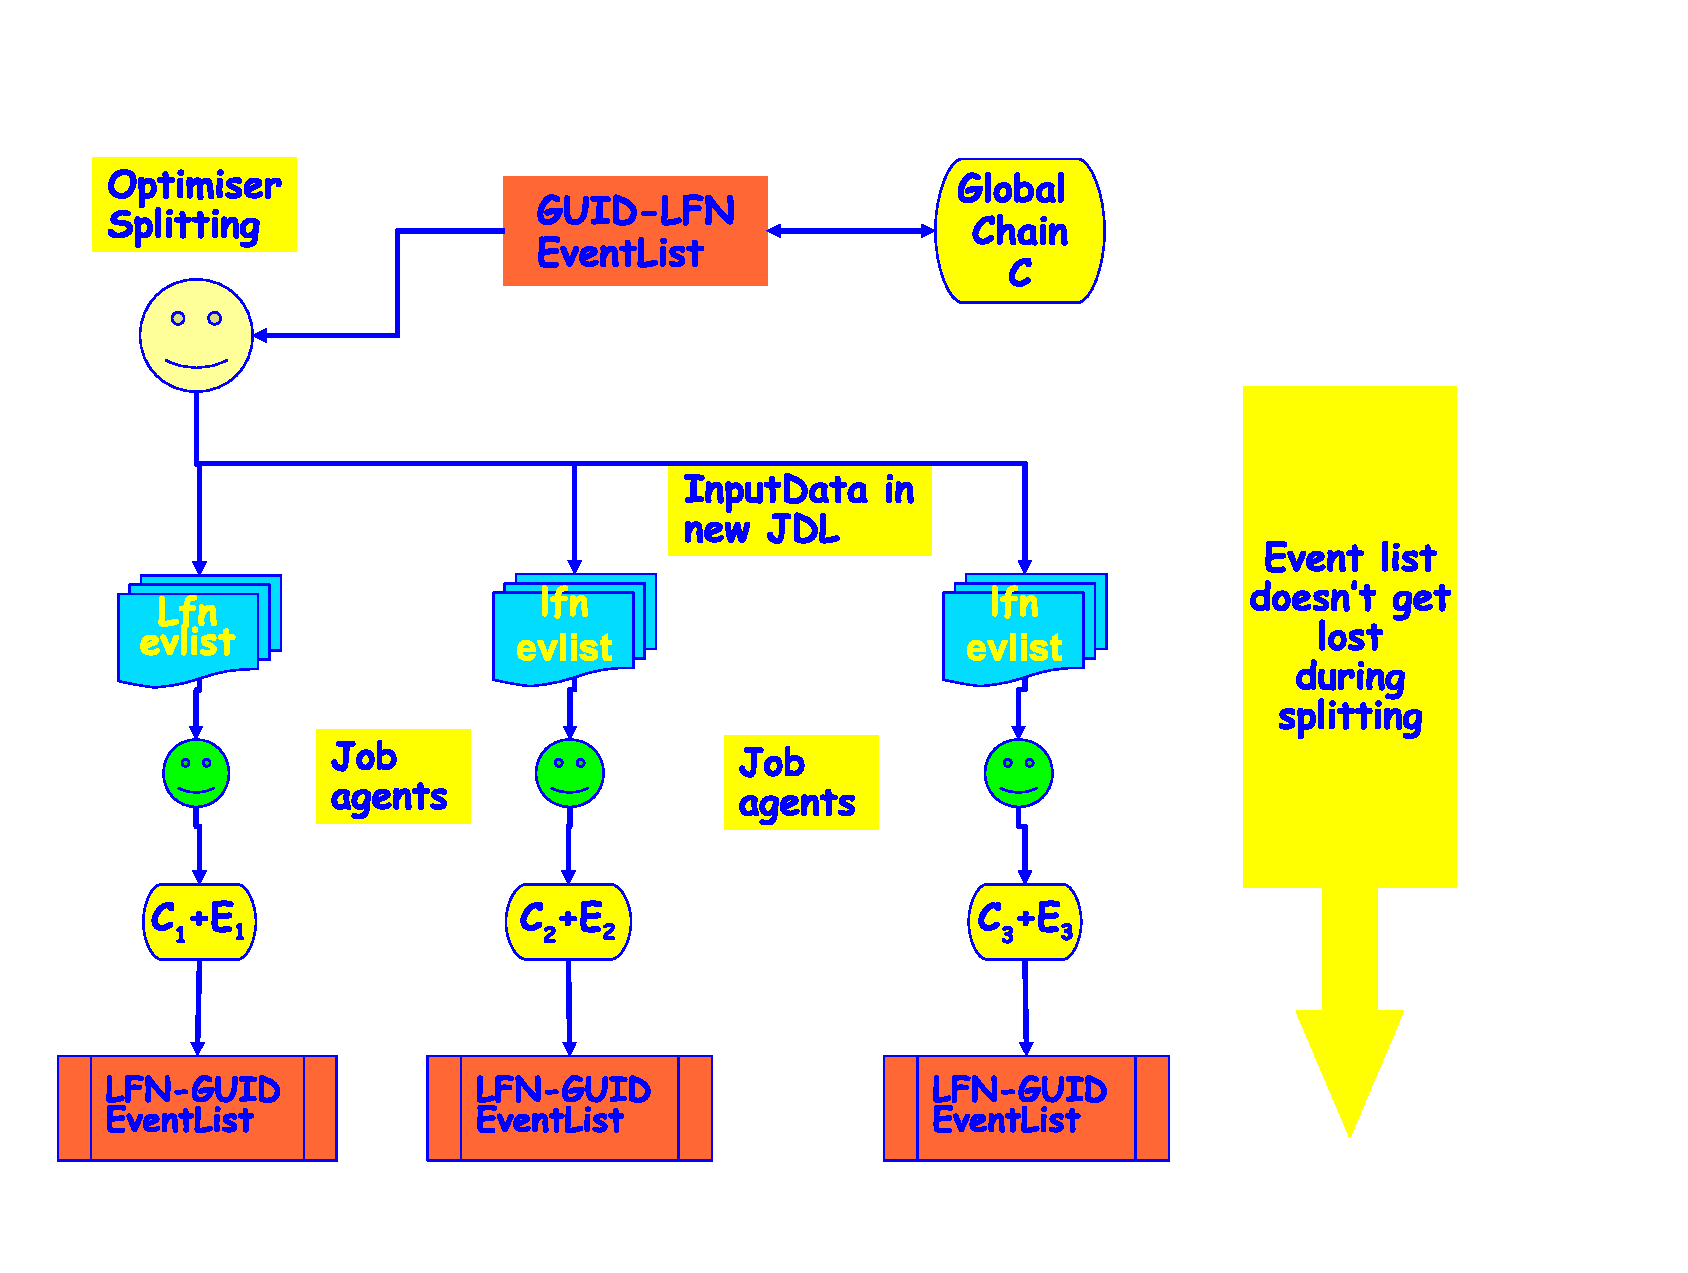
\includegraphics[width=0.7\textheight]{figures/Batch2.eps}
\end{center}
\caption{A schematic view of the flow of the analysis procedure in a batch session using the \tag. Following the arrows, we have the initial xml collection which is created by the {\ttfamily \textbf{IlcTagAnalysis}} class listed in the jdl as an {\ttfamily \textbf{InputDataCollection}} field. The optimizer takes this xml once the master job is submitted and splits it into several sub-jobs while in parallel writing new xml collections on every worker node. These xml collections hold the information about the events that satisfy the imposed selection criteria, grouped by file: the analysis is performed only on these events on every worker node.}
\label{Note:FigAnalsysisFlowBatchTag}
\end{figure}

The next step will be, as in the previous section, to create a jdl file inside of which this newly created xml collection will be define as an {\ttfamily \textbf{InputDataCollection}} field. Then we once again submit the job and the optimizer parses the xml and splits the master job into several sub-jobs. In parallel, a new xml collection is written on every site, containing the information about the files that will be analyzed on every worker node as well as the corresponding list of events that satisfy the imposed selection criteria for every file. Thus, on every worker node we will analyze the created chain along with the associated event list as described in Fig.\,\ref{Note:FigAnalsysisFlowBatchTag}. Once finished, we will get several output files over which we will have to loop with a post process in order to merge them \cite{Note:RefIlcenTutorial,Note:RefEventTagWeb}.

In the following paragraphs we will provide some practical information about the batch sessions, starting from the files needed to submit a job, what is the jdl syntax etc.

%________________________________________________________
\subsection{Files needed}

The files needed in order to submit a batch job are listed below \cite{Note:RefIlcenTutorial}:

\begin{itemize}
\item \textbf{Executable}: This is a file that should be stored under the \$HOME/bin AliEn directory of each user. It is used to start the ROOT/IlcRoot session on every worker node. Users can always use existing executables that can be found under /bin. An example is given below.
\item \textbf{Par file}: A {\ttfamily par file} is a tarball containing the header files and the source code of IlcRoot, needed to build a certain library. It is used in the case where we do not want to launch ilcroot but instead we want to be flexible by launching root along with the corresponding ilcroot library (e.g root and the libESD.so). It is not compulsory although it is recommended to use a par file in an analysis.
\item \textbf{Macro}: It is the file that each user needs to implement. Inside the macro we setup the par file (in case we use it) and we load the needed libraries. Then we open the input xml collection and convert it into a chain of trees. Finally we process this chain with a selector. A snapshot of such a file has already been given in section \ref{Note:INTERACTIVE}.
\item \textbf{XML collection}: This is the collection created either by directly querying the file catalog (in the case where we don't use the \tag) or by querying the \tag (case described in the previous paragraph).
\item \textbf{JDL}: This is a compulsory file inside of which we should describe the input/output files as well as the packages that we are going to use. A detailed description about the JDL fields is provided in the next lines.
\end{itemize}

\textbf{Example of an ``executable''}
\begin{lstlisting}[language=bash]
  #!/bin/bash
  
  echo ===========================
  echo $PATH
  echo $LD_LIBRARY_PATH
  echo ==========================
  
  root -b -x runProcess.C;
\end{lstlisting}

%________________________________________________________
\subsection{JDL syntax}

In this section we will try to describe in detail the different jdl fields \cite{Note:RefGSHELL}.

\begin{itemize}
\item \textbf{Executable}: It is the only compulsory field of the JDL where we give the logical file name (lfn) of the executable that should be stored in /bin or \$VO/bin or \$HOME/bin. A typical syntax can be: \\{\ttfamily \textbf{Executable="balance.sh";}}.

\item \textbf{Packages}: The definition of the packages that will be used in the batch session. The different packages installed can be found by typing \textbf{packages} in the AliEn shell \cite{Note:RefGSHELL}. A typical syntax can be: \\{\ttfamily \textbf{Packages={"APISCONFIG::V2.2","ROOT::v5-13-04a"};}}.

\item \textbf{Jobtag}: A comment that describes the job. A typical syntax can be: \\{\ttfamily \textbf{Jobtag={"comment:Balance Function for pp@0.9TeV"};}}.

\item \textbf{InputFile}: In this field we define the files that will be transported to the node where the job will run and are needed for the analysis. A typical syntax can be: \\{\ttfamily \textbf{InputFile= {\\"LF:/ilc/cern.ch/user/p/pchrist/Tutorial/BATCH/IlcAnalysisTaskPt.cxx",\\"LF:/ilc/cern.ch/user/p/pchrist/Tutorial/BATCH/IlcAnalysisTaskPt.h",\\"LF:/ilc/cern.ch/user/p/pchrist/Tutorial/BATCH/ESD.par", \\"LF:/ilc/cern.ch/user/p/pchrist/Tutorial/BATCH/ANALYSIS\_NEW.par", \\"LF:/ilc/cern.ch/user/p/pchrist/Tutorial/BATCH/demoBatch.C",\\"LF:/ilc/cern.ch/user/p/pchrist/Tutorial/BATCH/runProcess.C"};}}.

\item \textbf{InputData}: This field, when defined, requires that the job will be executed in a site close to files specified here. This is supposed to be used in the case where you don't want to use a collection of files. It should be pointed out that it is not really practical because it implies that each user writes a large number of lines in the jdl, thus making it difficult to handle. It should be pointed out that this approach can be useful in the case where we use a few files. A typical syntax can be: \\{\ttfamily \textbf{InputFile= {\\"LF:/ilc/cern.ch/user/p/pchrist/Tutorial/PDC06/001/IlcESDs.root"}}}.

\item \textbf{InputDataList}: This is the name of the xml file created by the job agent after the job has been split, containing the lfn of the files of the closest storage element. A typical syntax can be: \\{\ttfamily \textbf{InputDataList="pp.xml";}}.

\item \textbf{InputDataListFormat}: The format of the previous field. It can be either ``xml-single'' where we imply that every xml entry corresponds to one file or ``xml-group'' where we imply that a new set of files starts every time the base filename appears (e.g. xml containing IlcESDs.root, Kinematics.root, gilc.root). In the context of this note, where we analyze only ESDs and not the generator information, we should use the first option. A typical syntax can be: \\{\ttfamily \textbf{InputDataListFormat="xml-single";}}. 

\item \textbf{OutputFile}: Here we define the files that will be registered in the file catalog once the job finishes. If we don't define the storage element, then the files will be registered in the default one which at the moment is Castor2 at CERN. A typical syntax can be: \\{\ttfamily \textbf{OutputFile={"stdout@ILC::CERN::Castor2",\\"stderr@ILC::CERN::Castor2","*.root@ILC::CERN::Castor2"};}}. 

\item \textbf{OutputDir}: Here we define the directory in the file catalog under which the output files and archives will be stored. A typical syntax can be: \\{\ttfamily \textbf{OutputDir="/ilc/cern.ch/user/p/pchrist/Balance/output";}}.

\item \textbf{OutputArchive}: Here we define the files that we want to be put inside an archive. It is recommended that the users use this field in order to place all their output files in such an archive which will be the only registered file after a job finishes. This is essential in the case of storage systems such as Castor which are not effective in handling small files. A typical syntax can be: \\{\ttfamily \textbf{OutputArchive={"logarchive:stdout,stderr,*.log@Ilc::CERN::scratch",\\"rootarchive.zip:gilc.root,geometry.root,Kinematics.root,\\TrackRefs.root,IlcESDs.root,IlcESDfriends.root,check.root,Run*.root\\@Ilc::CERN::castor2"};}}.

\item \textbf{Validationcommand}: Specifies the script to be used as a validation script (used for production). A typical syntax can be: \\{\ttfamily \textbf{Validationcommand =\\"/ilc/cern.ch/user/a/ilcprod/prod2006/configspp/validation.sh";}}.

\item \textbf{Email}: If this field is defined, then you'll be informed that your job has finished from an e-mail. A typical syntax can be: \\{\ttfamily \textbf{Email="Panos.Christakoglou@cern.ch";}}.

\item \textbf{TTL}: One of the important fields of the JDL. It allows the user to define the maximum time in seconds the job will run. This field is used by the optimizer for the ordering and the assignment of the priority for each job. Lower value of TTL provides higher probability for the job to run quickly after submission. If the running time exceeds the one defined in this field, then the job is killed automatically. The value of this field should not exceed 100000 sec. A typical syntax can be: \\{\ttfamily \textbf{TTL = "21000";}}. 

\item \textbf{Split}: Used in the case we want to split our master job into several sub-jobs. Usually the job is split per storage element (se). A typical syntax can be: \\{\ttfamily \textbf{Split="se";}}.

\item \textbf{SplitMaxInputFileNumber}: Used to define the maximum number of files that will be analyzed on every worker node. A typical syntax can be: \\{\ttfamily \textbf{SplitMaxInputFileNumber="100";}}.

\end{itemize}

In summary, the following lines give a snapshot of a typical jdl:

\vspace{0.5 cm}
\textbf{Example of a JDL file}
\begin{lstlisting}[language=bash]
  # this is the startup process for root
  Executable="balance.sh";
  Jobtag={"comment:Balance Function for pp@0.9TeV"};
  
  # we split per storage element
  Split="se";
  
  # we want each job to read 100 input files
  SplitMaxInputFileNumber="100";
  
  # this job has to run in the ANALYSIS partition
  Requirements=( member(other.GridPartitions,"Analysis") );
  
  # we need ROOT and the API service configuration package
  Packages={"APISCONFIG::V2.2","ROOT::v5-13-04a"};

  # Estimation of the running time of the job
  TTL = "21000";
  
  # The xml file written by the job agent
  InputDataList="pp.xml";
  
  # ROOT requires the collection file in the xml-single format
  InputDataListFormat="xml-single";
  
  # This is our collection file containing the files to be analyzed
  InputDataCollection=
  "LF:/ilc/cern.ch/user/p/pchrist/Balance/xml/pp900.xml,nodownload";
  
  # These are the input files that will be registered in the job's sandbox
  InputFile={
  "LF:/ilc/cern.ch/user/p/pchrist/Tutorial/BATCH/IlcAnalysisTaskPt.cxx",
  "LF:/ilc/cern.ch/user/p/pchrist/Tutorial/BATCH/IlcAnalysisTaskPt.h",
  "LF:/ilc/cern.ch/user/p/pchrist/Tutorial/BATCH/ESD.par", 
  "LF:/ilc/cern.ch/user/p/pchrist/Tutorial/BATCH/ANALYSIS_NEW.par", 
  "LF:/ilc/cern.ch/user/p/pchrist/Tutorial/BATCH/demoBatch.C",
  "LF:/ilc/cern.ch/user/p/pchrist/Tutorial/BATCH/runProcess.C"};
  
  # These are the files inside the output archive
  OutputArchive={"log_archive:stdout,stderr@Ilc::CERN::se01",
    "root_archive.zip:*.root@Ilc::CERN::castor2"};
  
  # Output directory
  OutputDir="/ilc/cern.ch/user/p/pchrist/Balance/output";
  
  # email
  Email="Panos.Christakoglou@cern.ch";
  
\end{lstlisting}


%________________________________________________________
\subsection{Job submission - Job status}

After creating the jdl and registering all the files needed, we are ready to submit our batch job \cite{Note:RefGSHELL}. This can be done by typing: {\ttfamily \textbf{submit $<filename>$.jdl}} at the AliEn shell prompt. If there is no mistake in our JDL, the job will be assigned a JOBID. We can always see what are the jobs submitted by a certain user by typing {\ttfamily top -user $<username>$}. Later on, we can check its status by typing: {\ttfamily \textbf{ps -trace $<JOBID>$}}. The different states are:

\begin{itemize}

\item \textbf{INSERTING}: The job is waiting to be processed by the optimizer.
\item \textbf{SPLITTING}: The optimizer starts splitting the job if this is requested in the JDL.
\item \textbf{SPLIT}: Several sub-jobs were created from the master job.
\item \textbf{WAITING}: The job is waiting to be assigned to a job agent that fulfills its requirements.
\item \textbf{ASSIGNED}: A job agent is about to pick up this job.
\item \textbf{STARTED}: The job agent is preparing the input sandbox and transferring the files listed in the {\ttfamily \textbf{InputFile}} field.
\item \textbf{RUNNING}: The executable has started running.
\item \textbf{SAVING}: The executable has finished running and the job agent saves the output to the specified storage elements.
\item \textbf{SAVED}: The agent has successfully stored all the output files which are not available yet in the file catalog.
\item \textbf{DONE}: The central optimizer has registered the output in the catalog.

\end{itemize}

Finally, as long as a job status has turned into \textbf{RUNNING}, a user can check its stdout and stderr by typing: {\ttfamily \textbf{spy $<JOBID>$ stdout}} and {\ttfamily \textbf{spy $<JOBID>$ stderr}} at the AliEn prompt.


%________________________________________________________
\subsection{Merging the output}

Assuming that everything worked out and that the status of the job we had submitted has turned to {\ttfamily DONE}, we are ready to launch the post process that will access the different output files from every sub-job and merge them. We will concentrate in the case where the output files contain simple histograms (case which may represent the majority of the physics analyses). If the output files contain other analysis objects, then we should provide our own merge functions. The following lines give a snapshot of a sample macro that deals with this procedure:

\vspace{0.5 cm}
\textbf{Macro that merges output files containing ROOT histograms}
\begin{lstlisting}[language=C++]
  histomerge(const char* path, const char* pattern, const char* outfile=0){
    //Connect to ROOT's API since we need to access Grid stored files
    if(!gGrid) {
      TGrid::Connect("alien://");
    }
    
    //Create a TGridResult from the arguments of the function
    TGridResult* result = gGrid->Query(path,pattern);

    //Create a TFileMarger object and open an output file the name of which 
    //will be the third argument of the function
    TFileMerger m;
    if(outfile) m.OutputFile(outfile);
    Int_t i=0;
    TString fName = 0x0;

    //loop over the TGridResult entries and add the found files in the 
    //TFileMerger
    while (result->GetKey(i,"turl")) {
      fName = result->GetKey(i,"turl");
      cout<<fName<<endl;
      m.AddFile(fName);
      i++;
    }

    //Merge the output files
    if(i) m.Merge();
  }
\end{lstlisting}

The function needs three arguments:

\begin{itemize}
\item {\ttfamily path:} The file catalog path of the master job. It can be the {\ttfamily OutputDir} field if it is defined in the jdl or the {\ttfamily /proc/$<username>/<JOBID>$} if not.
\item {\ttfamily pattern:} This argument refers to the output file we create inside our selector.
\item {\ttfamily outfile:} This is the name of the output file that will be stored in our local working directory.
\end{itemize}

Finally, in order to run the macro we launch ROOT and invoke the following commands: \\
\\
{\ttfamily root [0] .L histomerge.C}\\
\\
{\ttfamily root [1] histomerge($<OutputDirPath>,<pattern>,<mergefile>$)}\\
\\

All the needed files to run these examples can be found inside the PWG2 module of IlcRoot under the AnalysisMacros/Batch directory.

